\documentclass[cjk]{beamer}

\usepackage[]{xeCJK,fontspec}
\setCJKmainfont{FandolSong}%{SimSun}
\setmainfont{CMU Serif}
\setsansfont{CMU Sans Serif}
\setmonofont{Sarasa Fixed SC}
%\setCJKmainfont{叶根友疾风劲草}
\setCJKfamilyfont{song}{FandolSong}
\newcommand{\song}{\CJKfamily{song}}
\setCJKfamilyfont{kaiti}{FandolKai}
\newcommand{\kaiti}{\CJKfamily{kaiti}}
\setCJKfamilyfont{heiti}{FandolHei}
\newcommand{\heiti}{\CJKfamily{heiti}}
%\usefonttheme[onlymath]{serif}
\usepackage{indentfirst}

%\usepackage[screen,panelright,gray,paneltoc,sectionbreak]{pdfscreen}
  %缺省状态为Blue,学术报告推荐采用"gray"。
%\usepackage{amsmath,amssymb,amsfonts}
%\usepackage[indentfirst]{titlesec}
%\usepackage{fancyvrb}
%\usepackage{graphicx}
%\usepackage{times}
%\usepackage{type1cm}
%\usepackage{geometry}
%\usepackage{hyperref}
%\usepackage[display]{texpower}
%\usepackage{hypbmsec}
%\usepackage{manfnt}
%\usepackage{pause}
%\usepackage{bbding}
%\usepackage{beamerthemeshadow} %该为一现成的模板,在 MiKTeX\texmf\tex\latex\beamer\themes\theme下面有很多

%\paneloverlay{./Overlays/but.pdf}
\usetheme{Warsaw} %{Madrid}
\usepackage{graphics,tcolorbox}
\usepackage{graphicx,xcolor,xcolor-solarized}
\usepackage{ amssymb }
\usepackage{amsmath,amssymb,amsfonts}
\usepackage{manfnt}
\newcommand{\chuhao}{\fontsize{52pt}{\baselineskip}\selectfont}

\mode<article> % 仅应用于article版本
{
  \usepackage{beamerbasearticle}
  \usepackage{fullpage}
  \usepackage{hyperref}
}



\usefoottemplate{\vbox{%
\tinycolouredline{structure!120}%
 {\color{white}\textbf{\insertshortauthor\hfil%
 \insertshorttitle}\hfil   \insertframenumber{} / \inserttotalframenumber}%\hfil
}}
\makeatother
\newtheorem{原因}{{原因}}[section]
\newtheorem{定义2.2}{{定义2.2}}[section]
\newtheorem{引理2.1}{{引理2.1}}[section]
\newtheorem{引理2.2}{{引理2.2}}[section]
\newtheorem{定理2.1}{{定理2.1}}[section]
\newtheorem{定理2.2}{{定理2.2}}[section]
\newtheorem{为什么追求高精度?}{{为什么追求高精度?}}[section]
%\newtheorem{definition}{{definition}}[section]
\newtheorem{lem}{{引理}}[section]
\newtheorem{remark}{{注记}}[section]
\newtheorem{dingyi}{{定义}}[section]
\renewcommand{\figurename}{图}


%%%%%%%%%%%%%%%%%%%%%%%%%%%%%%%%%%%%%%%%%%%%%%%%%%%%%%%%%%%%%%%%%%%%%%%%%%%%%%%%%%%%%%%%%%%%%%%%%%%%%%%%%
%                                           定制幻灯片---幅面、标志、底板、主页、按钮行距等             %
%%%%%%%%%%%%%%%%%%%%%%%%%%%%%%%%%%%%%%%%%%%%%%%%%%%%%%%%%%%%%%%%%%%%%%%%%%%%%%%%%%%%%%%%%%%%%%%%%%%%%%%%%
%\margins{15mm}{15mm}{15mm}{15mm}            %定义页边的空白尺寸,\margins{left}{right}{top}{bottom}。
%\screensize{180mm}{240mm}                   %定义屏幕尺寸,\screensize{height}{width},通常为180mm*240mm。
%\panelwidth=36mm                           %定义导航面板的宽度,缺省为幻灯片宽度的15%。
%\emblema{./Images/ecnu.png}                   %在导航面板加入图片。
%\overlay{./Overlays/overlay\theslideoverlay}  %多种overlay图形切换。注释该行,将得到无框SLIDE效果。
%\overlay{./Overlays/overlay1.pdf}            %在幻灯片中只用一种图片,\overlay{hgraphic file namei},是上一行的变体。
%\backgroundcolor{white}                    %\overlay被注视后的背景颜色。
%\paneloverlay{./Overlays/but.pdf}             %加入导航面板*.pdf。
%\urlid{math.ecnu.edu.cn/~latex}             %主页链接。
%\def\pfill{\vskip8pt}                       %导航面板项目行行距。
%\bottombuttons  %\nobottombuttons          %底部按钮开关。
%\topbuttons  %\notopbuttons                %顶部按钮开关。

%%%%%%%%%%%%%%%%%%%%%%%%%%%%%%%%%%%%%%%%%%%%%%%%%%%%%%%%%%%%%%%%%%%%%%%%%%%%%%%%%%%%%%%%%%%%%%%%%%%%%%%%%
%                                           定制幻灯片---导航面板目录中文化                             %
%%%%%%%%%%%%%%%%%%%%%%%%%%%%%%%%%%%%%%%%%%%%%%%%%%%%%%%%%%%%%%%%%%%%%%%%%%%%%%%%%%%%%%%%%%%%%%%%%%%%%%%%%



\title{避障跟人小车\quad 开题报告}
\author{组员:郭子笑\ 仇琨元\ 郑磊\ 李昀镀}%剩下两个人也加进去
\date{\footnotesize \vspace{5mm}2020.10.16}


\begin{document} %申明文档的开始
%\begin{CJK*}{GBK}{li}
%\begin{CJK*}{GBK}{song}     %CJK:支持中文

    \begin{frame} %beamer里重要的概念,每个frame定义一张page

        \titlepage

    \end{frame}

    \begin{frame}
     \frametitle{目录}
     \begin{enumerate}
\normalsize

%     \item \href{./figure/com.pdf}{导心系统回顾}\\
     \item 项目背景\\
智能小车\\
OpenCV图像识别库\\
     \qquad\\
     \item 主要设计目标\\
基本任务\\
基本参数指标\\
     \qquad\\
     \item 总体实现方案\\
总体流程图\\
模块流程图\\
     \qquad
     \item 拓展任务\\
     \qquad\\
 \item 致谢\\
%   \item \href{./figure/Boris.pdf}{Boris algorithm 数值算例}\\%3
%     \qquad\\
%     \item Boris algorithm 是否是共轭辛的\\%1:系统本身的稳定性:研究系统本身的性质,找出稳定的区域
%数值格式的稳定性:有效控制计算过程中数据大小,使其再有限步计算中范数相对有界\\
     \end{enumerate}
%     \tableofcontents
    \end{frame}



\frame{ \frametitle{项目背景}
\begin{tcolorbox}[colback=gray!10,%gray background
     colframe=red!75!black,% black frame colour
     %width=8cm,% Use 8cm total width,
     arc=1mm, auto outer arc,
     boxrule=0.5pt,
    ]
A.{\heiti 智能小车}
\end{tcolorbox}
\vspace{5mm}
\normalsize
~~~~~~本项目以电动智能小车为背景来研究智能化技术。智能小车集单片机技术、无线通讯技术、多种传感器信号的检测技术为一体,通过车载微控制器与传感器实现实时采集传感器信号、分析外部环境信息、自动方向控制等功能,制作一个能够自主识别道路的模型汽车,可以跟随人体进行移动,并能在移动过程中绕开障碍物。
}
\frame{\frametitle{项目背景}
\begin{tcolorbox}[colback=gray!10,%gray background
     colframe=red!75!black,% black frame colour
     %width=8cm,% Use 8cm total width,
     arc=1mm, auto outer arc,
     boxrule=0.5pt,
    ]
    B.{\heiti OpenCV图像识别库}
\end{tcolorbox}
\vspace{5mm}
\normalsize
~~~~~~OpenCV是一个基于BSD许可(开源)发行的跨平台计算机视觉和机器学习软件库,可以运行在Linux({\kaiti \color[rgb]{0.93,0.38,0.12}树莓派})、Windows和Mac OS等常用操作系统上,无论是PC,手机还是各种嵌入式平台均可良好支持。OpenCV轻量级而且高效——此机器视觉库由一系列 C 函数和少量 C++ 类构成,同时提供了Python、MATLAB等语言的接口,便于与基于Python等语言的神经网络对接,实现了图像处理和计算机视觉方面的很多通用算法。
}
\frame{\frametitle{主要设计目标}
\begin{tcolorbox}[colback=gray!10,%gray background
     colframe=red!75!black,% black frame colour
     %width=8cm,% Use 8cm total width,
     arc=1mm, auto outer arc,
     boxrule=0.5pt,
    ]
A.{\heiti 基本任务}
\end{tcolorbox}
\vspace{5mm}
\normalsize
\begin{enumerate}
     \item 自动寻找并跟随人体前进,人移动时小车能跟随\\
     \item 避开随机摆放的障碍物,若避障过程中丢失目标能重新锁定人体\\
     \item 小车离人体距离较近时停止前进,距离拉远时继续跟踪\\
     \item 人移动时摄像头始终对准人体。\\
     \item 如果有多人在场小车只锁定上位机指定的人体目标\\
\end{enumerate}
}
\frame{\frametitle{主要设计目标}
\begin{tcolorbox}[colback=gray!10,%gray background
     colframe=red!75!black,% black frame colour
     %width=8cm,% Use 8cm total width,
     arc=1mm, auto outer arc,
     boxrule=0.5pt,
    ]
B.{\heiti 基本参数指标}
\end{tcolorbox}
\vspace{5mm}
\normalsize
\begin{enumerate}
     \item 在不大于4m*10m的场地(半个教室大小)寻找并锁定一个人体目标\\
     \item 不锁定人形纸板等干扰物,若有多人在场时只锁定其中一人\\
     \item 顺利避开所有障碍物,不与任何障碍物碰撞,若进入三面封闭的障碍物能自动原路退出\\
     \item 小车跟人并躲避障碍物移动到达终点总时间不大于1分钟,离人体距离30cm时停止\\
     \item 避障过程中摄像头始终对准目标\\
\end{enumerate}
}
\frame{\frametitle{总体实现流程图}
{\fontsize{8pt}{\baselineskip} 总体由人体检测、目标轮廓识别、跟踪信号产生、测距四部分组成。}
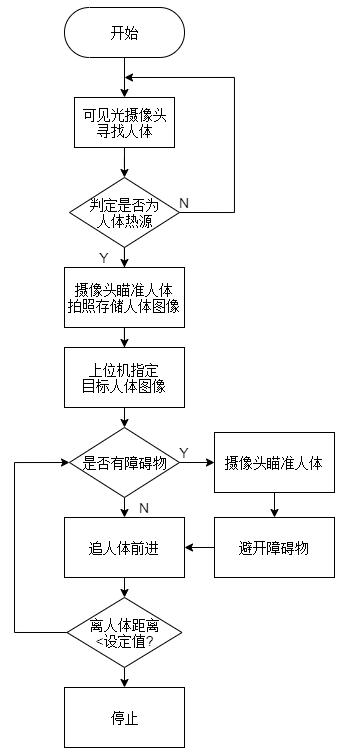
\includegraphics[height=7.4cm]{"./mainFlowChart.png"}
}
\frame{\frametitle{模块实现流程图}
\begin{tcolorbox}[colback=gray!10,%gray background
     colframe=yellow!46!red!75!black,% black frame colour
     %width=8cm,% Use 8cm total width,
     arc=1mm, auto outer arc,
     boxrule=0.8pt,
    ]
a.{\heiti\fontsize{8pt}{\baselineskip} 人体检测}
\end{tcolorbox}
{\fontsize{8pt}{\baselineskip} 通过PIR传感器或红外温度计({\kaiti \color[rgb]{0.93,0.38,0.12} AMG8833})检测人体散发的热量,或者使用雷达模块检测人体。}\\
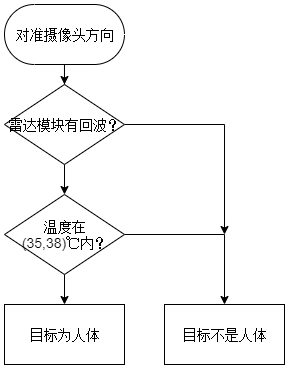
\includegraphics[height=4.6cm]{bodydetFlowChart.png}
}

\frame{\frametitle{模块实现流程图}
\begin{tcolorbox}[colback=gray!10,%gray background
     colframe=yellow!46!red!75!black,% black frame colour
     %width=8cm,% Use 8cm total width,
     arc=1mm, auto outer arc,
     boxrule=0.8pt,
    ]
b.{\heiti\fontsize{8pt}{\baselineskip} 目标轮廓识别}
\end{tcolorbox}
{\fontsize{8pt}{\baselineskip} 通过摄像头采集人体轮廓与颜色数据,然后给出各个人体照片的特征矢量。}\\
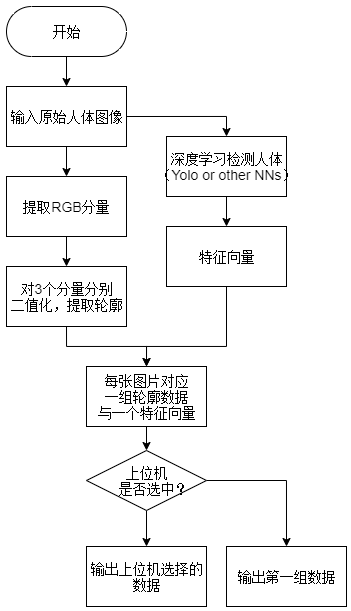
\includegraphics[height=4.6cm]{outlineextrFlowChart.png}
}

\frame{\frametitle{模块实现流程图}
\begin{tcolorbox}[colback=gray!10,%gray background
     colframe=yellow!46!red!75!black,% black frame colour
     %width=8cm,% Use 8cm total width,
     arc=1mm, auto outer arc,
     boxrule=0.8pt,
    ]
c.{\heiti\fontsize{8pt}{\baselineskip} 跟踪信号生成}
\end{tcolorbox}
{\fontsize{8pt}{\baselineskip} 通过摄像头实时采集人体轮廓与颜色数据,判定确认为目标后计算几何中心移动量,除以帧频得到速度}\\
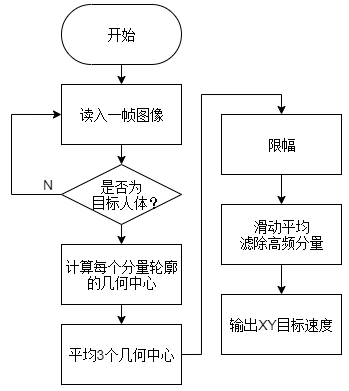
\includegraphics[height=4.6cm]{tgtvelFlowChart.png}
}
\frame{\frametitle{模块实现流程图}
\begin{tcolorbox}[colback=gray!10,%gray background
     colframe=yellow!46!red!75!black,% black frame colour
     %width=8cm,% Use 8cm total width,
     arc=1mm, auto outer arc,
     boxrule=0.8pt,
    ]
d.{\heiti\fontsize{8pt}{\baselineskip} 避障与原路退回}
\end{tcolorbox}
{\fontsize{8pt}{\baselineskip} 通过摄像头实时采集周围颜色数据,判定可通行区域的轮廓,结合人体的移动速度矢量给出移动方向。

该实现与(c)部分相似,使用OpenCV二值化抽取实时图像轮廓,滑动平均、色彩阈值滤波后给出可通行区域的中心坐标与边缘轮廓。在获取目标的移动方向后,若视野内与目标移动方向同向的位置存在可通行区域,小车即向该区域移动;若视野内只有一个可通行区域,小车即向唯一可通行路径移动;若视野内不存在可通行区域,小车将反向行驶直至出现可通行区域。

使用一个IMU测量并存储一定时间(数十秒)内小车行进的路径。}
}
\frame{\frametitle{拓展设计目标}
\begin{tcolorbox}[colback=gray!10,%gray background
     colframe=red!75!black,% black frame colour
     %width=8cm,% Use 8cm total width,
     arc=1mm, auto outer arc,
     boxrule=0.5pt,
    ]
A.{\heiti 发挥任务}
\end{tcolorbox}
\vspace{5mm}
\normalsize
\begin{enumerate}
     \item 上位机指定人体目标\\
     \item 通过图传模块或WiFi实时传输摄像头图像\\
     \item 随时切换为手动遥控\\
\end{enumerate}
}
\frame{\frametitle{拓展设计目标}
\begin{tcolorbox}[colback=gray!10,%gray background
     colframe=red!75!black,% black frame colour
     %width=8cm,% Use 8cm total width,
     arc=1mm, auto outer arc,
     boxrule=1pt,
    ]
X.{\heiti 远期目标}
\end{tcolorbox}
\vspace{5mm}
\normalsize
\begin{enumerate}
     \item 基于OpenCV的SLAM算法\\
     \item 使用多个雷达模块实现相控阵\\
     \item 自动瞄准的车载电磁炮\\
\end{enumerate}
\dots\quad\dots

}
\frame{
\begin{center}
\chuhao\fontspec[Variant = 2]{Harlow Solid Italic}{Thank You}
\end{center}
}
\end{document}
